% This file is generated by the MATLAB m-file laprint.m. It can be included
% into LaTeX documents using the packages graphicx, color and psfrag.
% It is accompanied by a postscript file. A sample LaTeX file is:
%    \documentclass{article}\usepackage{graphicx,color,psfrag}
%    \begin{document}% This file is generated by the MATLAB m-file laprint.m. It can be included
% into LaTeX documents using the packages graphicx, color and psfrag.
% It is accompanied by a postscript file. A sample LaTeX file is:
%    \documentclass{article}\usepackage{graphicx,color,psfrag}
%    \begin{document}% This file is generated by the MATLAB m-file laprint.m. It can be included
% into LaTeX documents using the packages graphicx, color and psfrag.
% It is accompanied by a postscript file. A sample LaTeX file is:
%    \documentclass{article}\usepackage{graphicx,color,psfrag}
%    \begin{document}% This file is generated by the MATLAB m-file laprint.m. It can be included
% into LaTeX documents using the packages graphicx, color and psfrag.
% It is accompanied by a postscript file. A sample LaTeX file is:
%    \documentclass{article}\usepackage{graphicx,color,psfrag}
%    \begin{document}\input{fig_P_f_vs_est_time_diff_snr_AWGN}\end{document}
% See http://www.mathworks.de/matlabcentral/fileexchange/loadFile.do?objectId=4638
% for recent versions of laprint.m.
%
% created by:           LaPrint version 3.16 (13.9.2004)
% created on:           03-Feb-2015 17:20:02
% eps bounding box:     24 cm x 18 cm
% comment:              
%
%\begin{psfrags}%
%\psfragscanon%
%
% text strings:
\psfrag{s01}[b][b]{\color[rgb]{0,0,0}\setlength{\tabcolsep}{0pt}\begin{tabular}{c}$\pfa$\end{tabular}}%
\psfrag{s02}[t][t]{\color[rgb]{0,0,0}\setlength{\tabcolsep}{0pt}\begin{tabular}{c}$\test$ = [ms]\end{tabular}}%
\psfrag{s06}[][]{\color[rgb]{0,0,0}\setlength{\tabcolsep}{0pt}\begin{tabular}{c} \end{tabular}}%
\psfrag{s07}[][]{\color[rgb]{0,0,0}\setlength{\tabcolsep}{0pt}\begin{tabular}{c} \end{tabular}}%
\psfrag{s08}[l][l]{\color[rgb]{0,0,0}pfal}%
\psfrag{s09}[l][l]{\color[rgb]{0,0,0}pfap}%
\psfrag{s10}[l][l]{\color[rgb]{0,0,0}pfau}%
\psfrag{s11}[l][l]{\color[rgb]{0,0,0}pfal}%
%
% xticklabels:
\psfrag{x01}[t][t]{2}%
\psfrag{x02}[t][t]{4}%
\psfrag{x03}[t][t]{6}%
\psfrag{x04}[t][t]{8}%
\psfrag{x05}[t][t]{10}%
\psfrag{x06}[t][t]{12}%
\psfrag{x07}[t][t]{14}%
%
% yticklabels:
\psfrag{v01}[r][r]{$10^{-4}$}%
\psfrag{v02}[r][r]{$10^{-3}$}%
\psfrag{v03}[r][r]{$10^{-2}$}%
\psfrag{v04}[r][r]{$10^{-1}$}%
%
% Figure:
%\resizebox{12cm}{!}{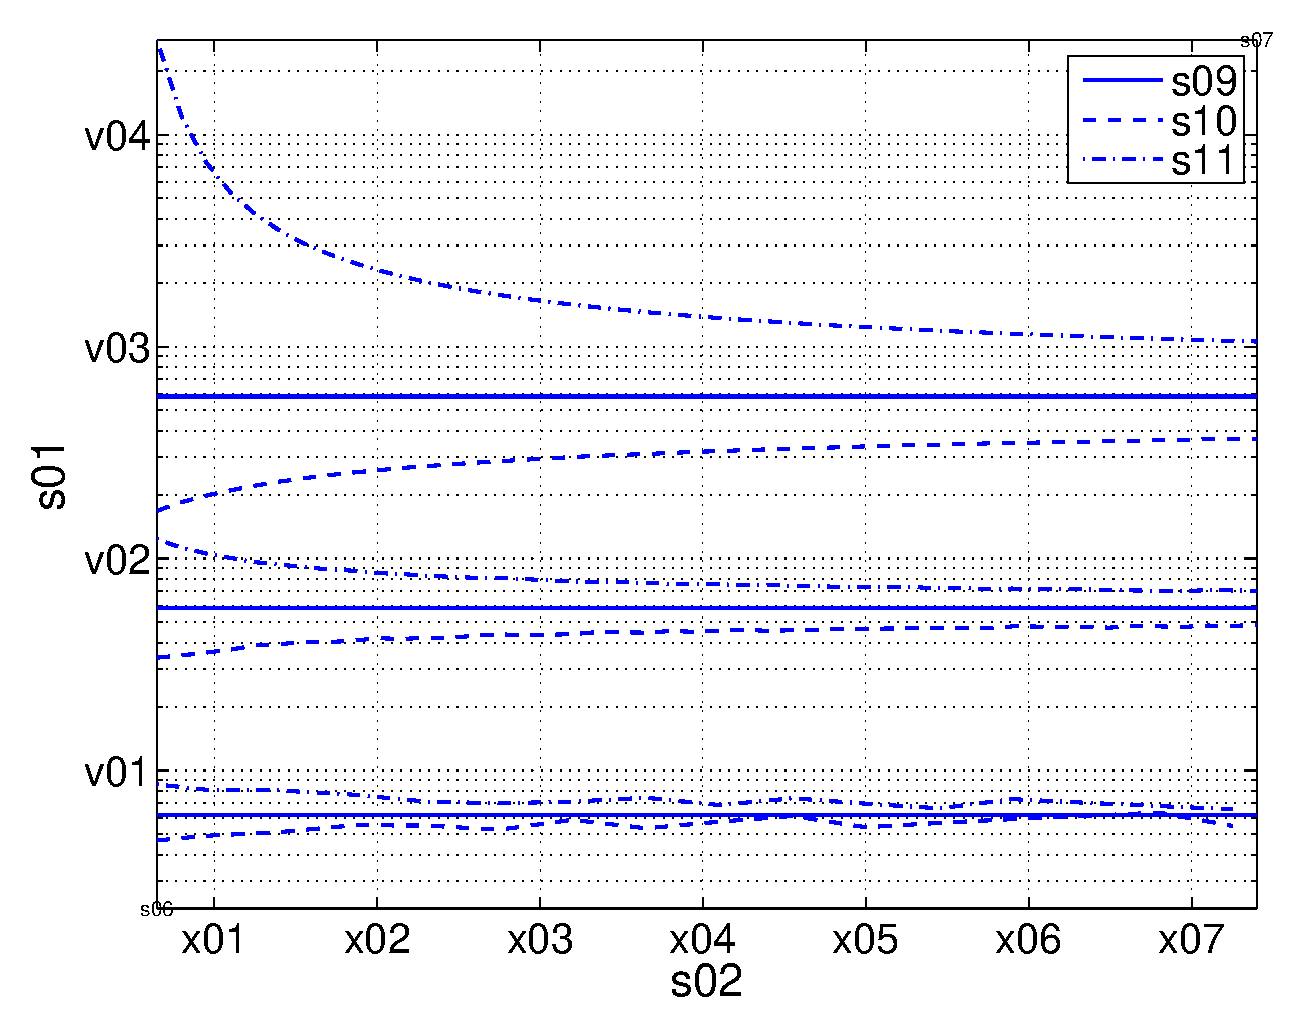
\includegraphics{fig_P_f_vs_est_time_diff_snr_AWGN.eps}}%
%\end{psfrags}%
%
% End fig_P_f_vs_est_time_diff_snr_AWGN.tex
\end{document}
% See http://www.mathworks.de/matlabcentral/fileexchange/loadFile.do?objectId=4638
% for recent versions of laprint.m.
%
% created by:           LaPrint version 3.16 (13.9.2004)
% created on:           03-Feb-2015 17:20:02
% eps bounding box:     24 cm x 18 cm
% comment:              
%
%\begin{psfrags}%
%\psfragscanon%
%
% text strings:
\psfrag{s01}[b][b]{\color[rgb]{0,0,0}\setlength{\tabcolsep}{0pt}\begin{tabular}{c}$\pfa$\end{tabular}}%
\psfrag{s02}[t][t]{\color[rgb]{0,0,0}\setlength{\tabcolsep}{0pt}\begin{tabular}{c}$\test$ = [ms]\end{tabular}}%
\psfrag{s06}[][]{\color[rgb]{0,0,0}\setlength{\tabcolsep}{0pt}\begin{tabular}{c} \end{tabular}}%
\psfrag{s07}[][]{\color[rgb]{0,0,0}\setlength{\tabcolsep}{0pt}\begin{tabular}{c} \end{tabular}}%
\psfrag{s08}[l][l]{\color[rgb]{0,0,0}pfal}%
\psfrag{s09}[l][l]{\color[rgb]{0,0,0}pfap}%
\psfrag{s10}[l][l]{\color[rgb]{0,0,0}pfau}%
\psfrag{s11}[l][l]{\color[rgb]{0,0,0}pfal}%
%
% xticklabels:
\psfrag{x01}[t][t]{2}%
\psfrag{x02}[t][t]{4}%
\psfrag{x03}[t][t]{6}%
\psfrag{x04}[t][t]{8}%
\psfrag{x05}[t][t]{10}%
\psfrag{x06}[t][t]{12}%
\psfrag{x07}[t][t]{14}%
%
% yticklabels:
\psfrag{v01}[r][r]{$10^{-4}$}%
\psfrag{v02}[r][r]{$10^{-3}$}%
\psfrag{v03}[r][r]{$10^{-2}$}%
\psfrag{v04}[r][r]{$10^{-1}$}%
%
% Figure:
%\resizebox{12cm}{!}{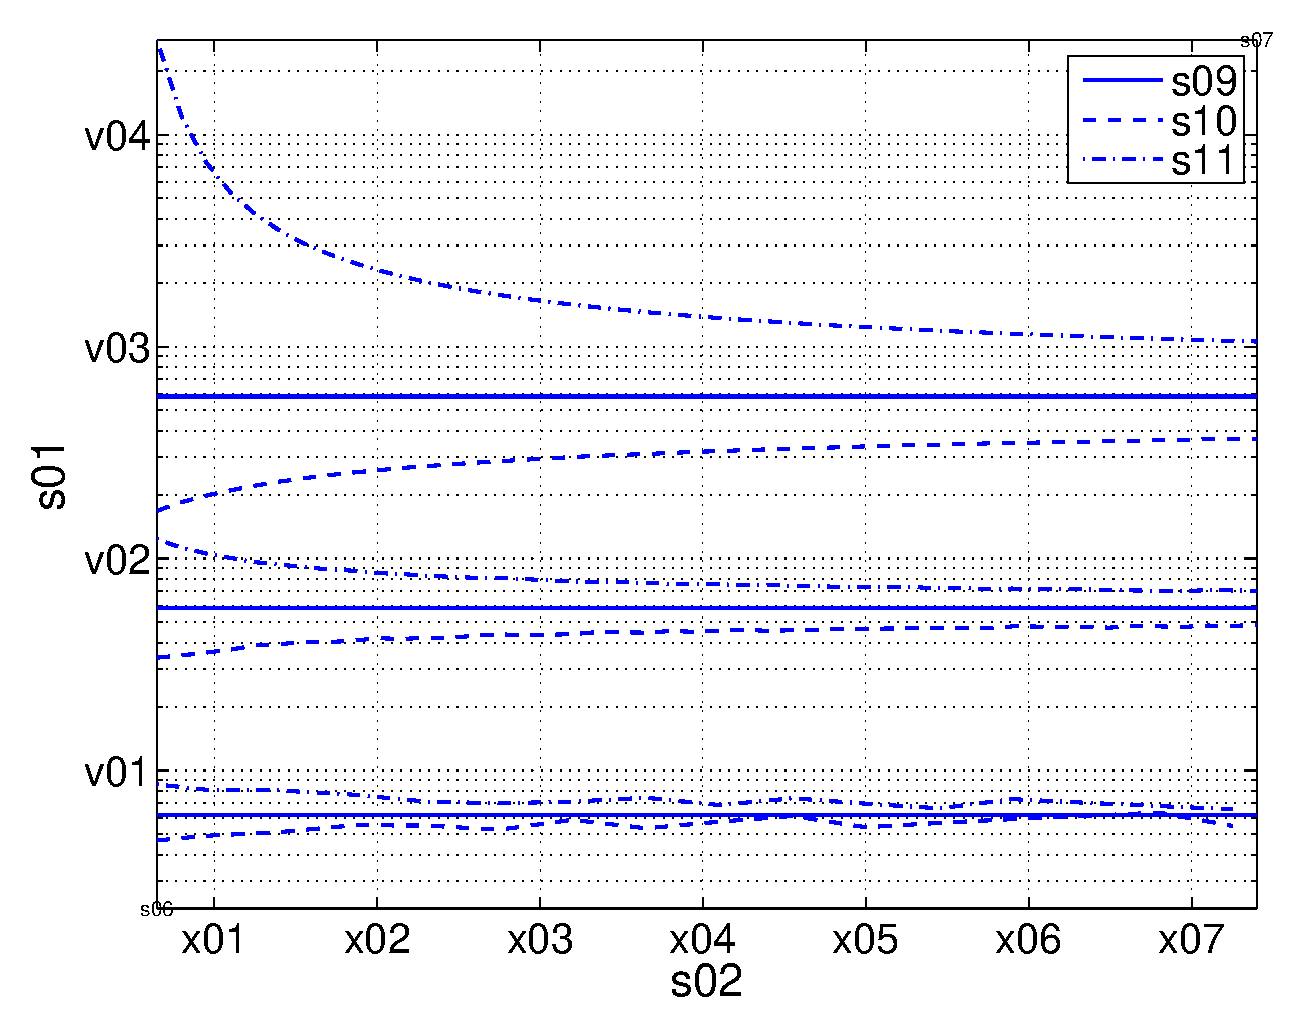
\includegraphics{fig_P_f_vs_est_time_diff_snr_AWGN.eps}}%
%\end{psfrags}%
%
% End fig_P_f_vs_est_time_diff_snr_AWGN.tex
\end{document}
% See http://www.mathworks.de/matlabcentral/fileexchange/loadFile.do?objectId=4638
% for recent versions of laprint.m.
%
% created by:           LaPrint version 3.16 (13.9.2004)
% created on:           03-Feb-2015 17:20:02
% eps bounding box:     24 cm x 18 cm
% comment:              
%
%\begin{psfrags}%
%\psfragscanon%
%
% text strings:
\psfrag{s01}[b][b]{\color[rgb]{0,0,0}\setlength{\tabcolsep}{0pt}\begin{tabular}{c}$\pfa$\end{tabular}}%
\psfrag{s02}[t][t]{\color[rgb]{0,0,0}\setlength{\tabcolsep}{0pt}\begin{tabular}{c}$\test$ = [ms]\end{tabular}}%
\psfrag{s06}[][]{\color[rgb]{0,0,0}\setlength{\tabcolsep}{0pt}\begin{tabular}{c} \end{tabular}}%
\psfrag{s07}[][]{\color[rgb]{0,0,0}\setlength{\tabcolsep}{0pt}\begin{tabular}{c} \end{tabular}}%
\psfrag{s08}[l][l]{\color[rgb]{0,0,0}pfal}%
\psfrag{s09}[l][l]{\color[rgb]{0,0,0}pfap}%
\psfrag{s10}[l][l]{\color[rgb]{0,0,0}pfau}%
\psfrag{s11}[l][l]{\color[rgb]{0,0,0}pfal}%
%
% xticklabels:
\psfrag{x01}[t][t]{2}%
\psfrag{x02}[t][t]{4}%
\psfrag{x03}[t][t]{6}%
\psfrag{x04}[t][t]{8}%
\psfrag{x05}[t][t]{10}%
\psfrag{x06}[t][t]{12}%
\psfrag{x07}[t][t]{14}%
%
% yticklabels:
\psfrag{v01}[r][r]{$10^{-4}$}%
\psfrag{v02}[r][r]{$10^{-3}$}%
\psfrag{v03}[r][r]{$10^{-2}$}%
\psfrag{v04}[r][r]{$10^{-1}$}%
%
% Figure:
%\resizebox{12cm}{!}{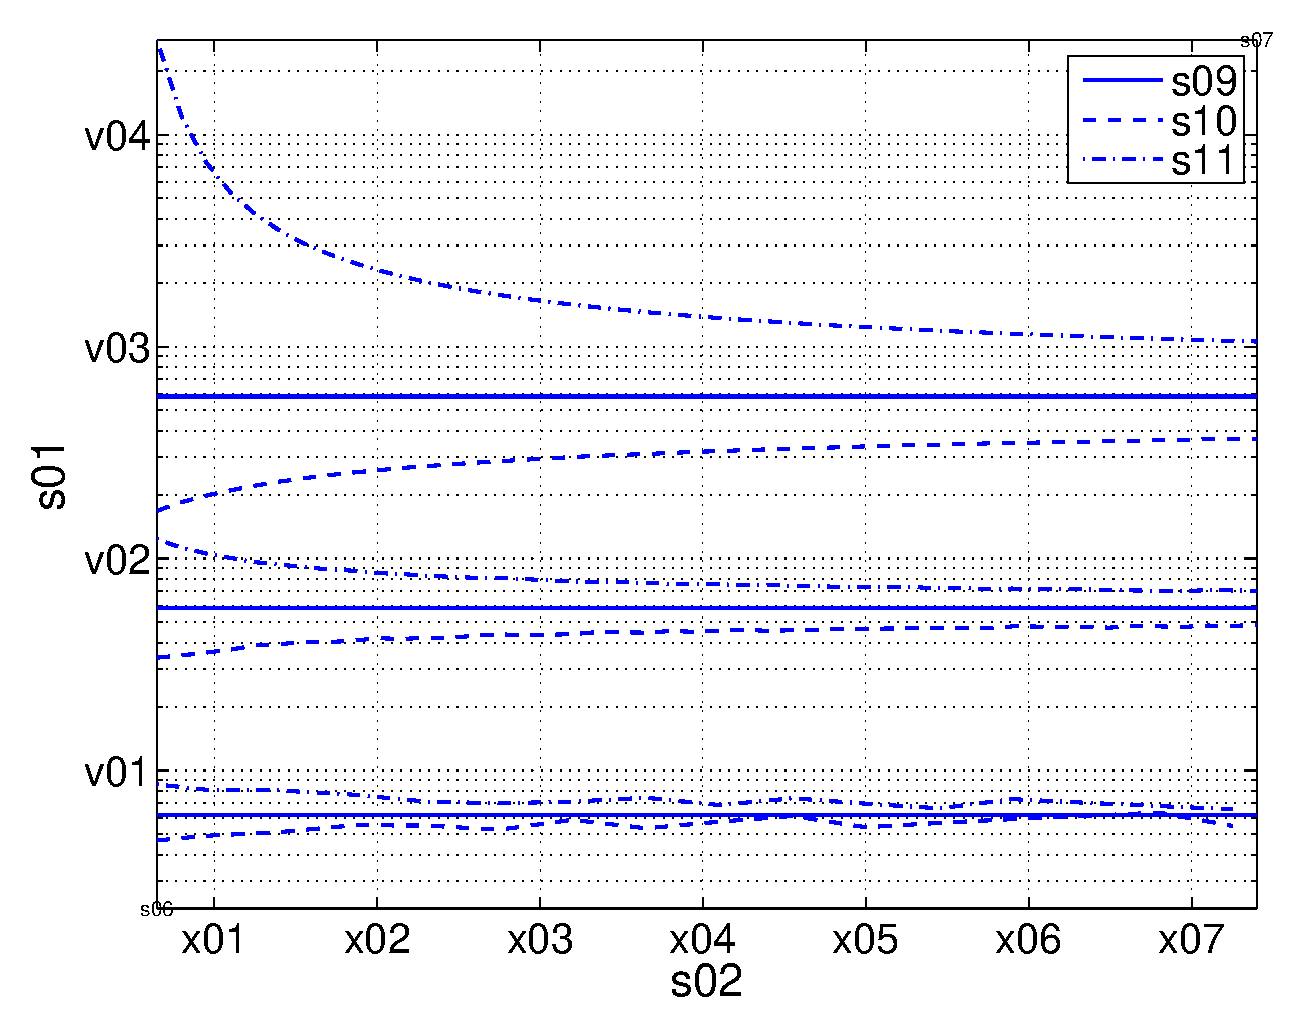
\includegraphics{fig_P_f_vs_est_time_diff_snr_AWGN.eps}}%
%\end{psfrags}%
%
% End fig_P_f_vs_est_time_diff_snr_AWGN.tex
\end{document}
% See http://www.mathworks.de/matlabcentral/fileexchange/loadFile.do?objectId=4638
% for recent versions of laprint.m.
%
% created by:           LaPrint version 3.16 (13.9.2004)
% created on:           03-Feb-2015 17:20:02
% eps bounding box:     24 cm x 18 cm
% comment:              
%
%\begin{psfrags}%
%\psfragscanon%
%
% text strings:
\psfrag{s01}[b][b]{\color[rgb]{0,0,0}\setlength{\tabcolsep}{0pt}\begin{tabular}{c}$\pfa$\end{tabular}}%
\psfrag{s02}[t][t]{\color[rgb]{0,0,0}\setlength{\tabcolsep}{0pt}\begin{tabular}{c}$\test$ = [ms]\end{tabular}}%
\psfrag{s06}[][]{\color[rgb]{0,0,0}\setlength{\tabcolsep}{0pt}\begin{tabular}{c} \end{tabular}}%
\psfrag{s07}[][]{\color[rgb]{0,0,0}\setlength{\tabcolsep}{0pt}\begin{tabular}{c} \end{tabular}}%
\psfrag{s08}[l][l]{\color[rgb]{0,0,0}pfal}%
\psfrag{s09}[l][l]{\color[rgb]{0,0,0}pfap}%
\psfrag{s10}[l][l]{\color[rgb]{0,0,0}pfau}%
\psfrag{s11}[l][l]{\color[rgb]{0,0,0}pfal}%
%
% xticklabels:
\psfrag{x01}[t][t]{2}%
\psfrag{x02}[t][t]{4}%
\psfrag{x03}[t][t]{6}%
\psfrag{x04}[t][t]{8}%
\psfrag{x05}[t][t]{10}%
\psfrag{x06}[t][t]{12}%
\psfrag{x07}[t][t]{14}%
%
% yticklabels:
\psfrag{v01}[r][r]{$10^{-4}$}%
\psfrag{v02}[r][r]{$10^{-3}$}%
\psfrag{v03}[r][r]{$10^{-2}$}%
\psfrag{v04}[r][r]{$10^{-1}$}%
%
% Figure:
%\resizebox{12cm}{!}{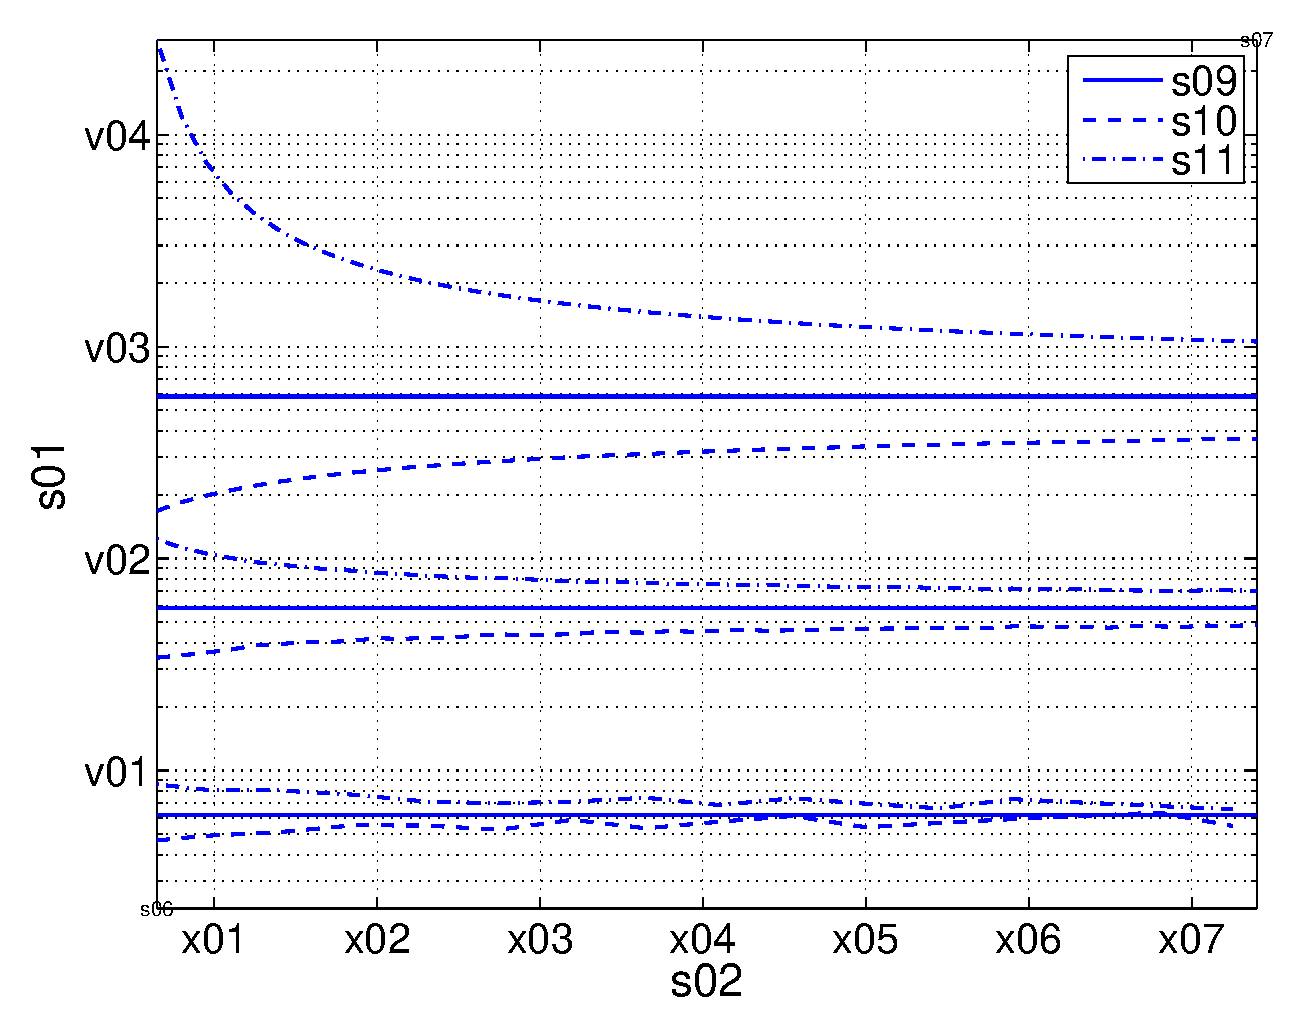
\includegraphics{fig_P_f_vs_est_time_diff_snr_AWGN.eps}}%
%\end{psfrags}%
%
% End fig_P_f_vs_est_time_diff_snr_AWGN.tex
